\documentclass[tikz,border=2mm]{standalone}
\usetikzlibrary{arrows.meta,calc,positioning}
\newcommand{\tikzsetnextfilename}[1]{}

\definecolor{iconblue}{RGB}{70,140,255}
\definecolor{softgreen}{RGB}{95,166,123}
\definecolor{softorange}{RGB}{226,145,67}
\definecolor{softred}{RGB}{205,88,84}

\tikzset{
  every node/.style={font=\sffamily},
  dot/.style={circle, draw=black, fill=white, line width=0.5pt,
    inner sep=0pt, minimum size=5pt},
  blue dot/.style={dot, fill=iconblue!75},
  edge/.style={line width=0.9pt, line cap=round, line join=round},
  path edge/.style={edge, draw=iconblue, line width=2pt, -{Stealth[length=4pt]}}
}

\begin{document}

\tikzsetnextfilename{ehrhart-order-polytopes}
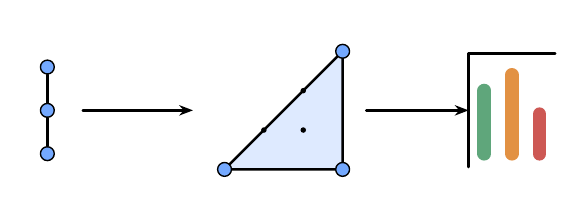
\begin{tikzpicture}[line cap=round,line join=round]
  \useasboundingbox (-3.25,-1.05) rectangle (3.25,1.05);

  \node[blue dot] (c1) at (-3.0,0.55) {};
  \node[blue dot] (c2) at (-3.0,0.0) {};
  \node[blue dot] (c3) at (-3.0,-0.55) {};
  \draw[edge] (c1) -- (c2) -- (c3);

  \fill[iconblue!18] (-0.75,-0.75) -- (0.75,-0.75) -- (0.75,0.75) -- cycle;
  \draw[edge] (-0.75,-0.75) -- (0.75,-0.75) -- (0.75,0.75) -- cycle;
  \foreach \p in {(-0.75,-0.75),(0.75,-0.75),(0.75,0.75)} {
    \node[blue dot] at \p {};
  }
  \foreach \x/\y in {-0.25/-0.25,0.25/-0.25,0.25/0.25} {
    \fill[black] (\x,\y) circle (1pt);
  }

  \draw[-{Stealth[length=5pt]}, edge] (-2.55,0) -- (-1.15,0);
  \draw[-{Stealth[length=5pt]}, edge] (1.05,0) -- (2.35,0);

  \draw[edge] (2.35,-0.72) -- (2.35,0.72) -- (3.45,0.72);
  \draw[softgreen, line width=5pt] (2.55,-0.55) -- (2.55,0.25);
  \draw[softorange, line width=5pt] (2.9,-0.55) -- (2.9,0.45);
  \draw[softred, line width=5pt] (3.25,-0.55) -- (3.25,-0.05);
\end{tikzpicture}

\tikzsetnextfilename{total-positivity-network}
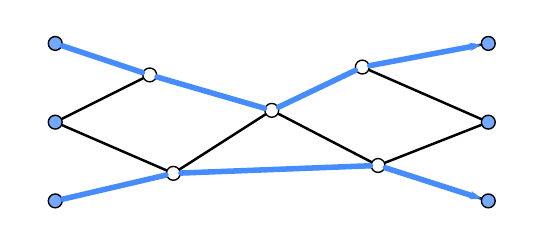
\begin{tikzpicture}[line cap=round,line join=round]
  \useasboundingbox (-3.1,-1.2) rectangle (3.1,1.2);

  \foreach \i/\y in {1/1,2/0,3/-1} {
    \node[blue dot] (s\i) at (-2.75,\y) {};
    \node[blue dot] (t\i) at (2.75,\y) {};
  }

  \node[dot] (a) at (-1.55,0.6) {};
  \node[dot] (b) at (-1.25,-0.65) {};
  \node[dot] (c) at (0.0,0.15) {};
  \node[dot] (d) at (1.15,0.7) {};
  \node[dot] (e) at (1.35,-0.55) {};

  \draw[edge] (s1) -- (a) -- (c) -- (d) -- (t1);
  \draw[edge] (s2) -- (a);
  \draw[edge] (s2) -- (b) -- (c);
  \draw[edge] (c) -- (e) -- (t2);
  \draw[edge] (b) -- (e) -- (t3);
  \draw[edge] (d) -- (t2);
  \draw[edge] (s3) -- (b);

  \draw[path edge] (s1) -- (a) -- (c) -- (d) -- (t1);
  \draw[path edge] (s3) -- (b) -- (e) -- (t3);
\end{tikzpicture}

\tikzsetnextfilename{coxeter-types-diagrams}
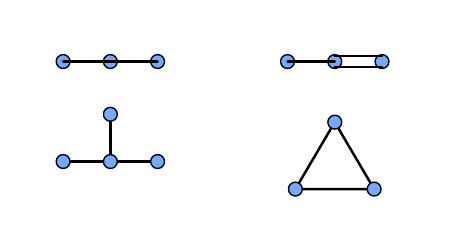
\begin{tikzpicture}[line cap=round,line join=round]
  \useasboundingbox (-2.6,-1.15) rectangle (2.6,1.15);

  \foreach \x in {-2.15,-1.55,-0.95} {
    \node[blue dot] at (\x,0.72) {};
  }
  \draw[edge] (-2.15,0.72) -- (-1.55,0.72) -- (-0.95,0.72);

  \foreach \x in {0.7,1.3,1.9} {
    \node[blue dot] at (\x,0.72) {};
  }
  \draw[edge] (0.7,0.72) -- (1.3,0.72);
  \draw[edge] (1.3,0.79) -- (1.9,0.79);
  \draw[edge] (1.3,0.65) -- (1.9,0.65);

  \node[blue dot] (d0) at (-1.55,-0.55) {};
  \node[blue dot] (d1) at (-2.15,-0.55) {};
  \node[blue dot] (d2) at (-0.95,-0.55) {};
  \node[blue dot] (d3) at (-1.55,0.05) {};
  \draw[edge] (d1) -- (d0) -- (d2);
  \draw[edge] (d0) -- (d3);

  \node[blue dot] (a1) at (0.8,-0.9) {};
  \node[blue dot] (a2) at (1.8,-0.9) {};
  \node[blue dot] (a3) at (1.3,-0.05) {};
  \draw[edge] (a1) -- (a2) -- (a3) -- (a1);

\end{tikzpicture}

\tikzsetnextfilename{qsym-nsym-zero-hecke}
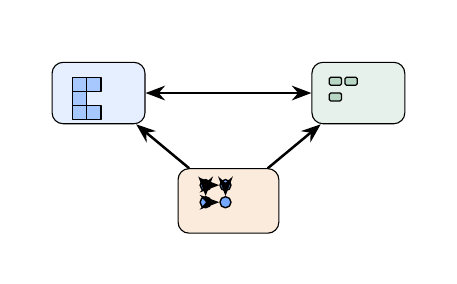
\begin{tikzpicture}[line cap=round,line join=round]
  \useasboundingbox (-2.55,-1.45) rectangle (2.55,1.45);

  \node[draw=black, rounded corners=4pt, fill=iconblue!14,
    minimum width=1.18cm, minimum height=0.78cm] (q) at (-1.65,0.62) {};
  \node[draw=black, rounded corners=4pt, fill=softgreen!16,
    minimum width=1.18cm, minimum height=0.78cm] (n) at (1.65,0.62) {};
  \node[draw=black, rounded corners=4pt, fill=softorange!18,
    minimum width=1.28cm, minimum height=0.82cm] (h) at (0,-0.75) {};

  \draw[edge, <->, >=Stealth] (q) -- (n);
  \draw[edge, ->, >=Stealth] (h) -- (q);
  \draw[edge, ->, >=Stealth] (h) -- (n);

  \begin{scope}[shift={(-1.98,0.82)}, scale=0.18]
    \foreach \x/\y in {0/0,1/0,0/-1,0/-2,1/-2} {
      \filldraw[fill=iconblue!48, draw=black, line width=0.45pt]
        (\x,\y) rectangle ++(1,-1);
    }
  \end{scope}
  \begin{scope}[shift={(1.28,0.82)}, scale=0.2]
    \foreach \x/\y/\c in {0/0/softgreen,1/0/softgreen,0/-1/softgreen} {
      \filldraw[fill=\c!45, draw=black, line width=0.45pt,
        rounded corners=0.5pt] (\x,\y) rectangle ++(0.78,-0.5);
    }
  \end{scope}
  \begin{scope}[shift={(-0.29,-0.55)}, scale=0.35]
    \node[blue dot, minimum size=4pt] (a) at (0,0) {};
    \node[blue dot, minimum size=4pt] (b) at (0.72,0) {};
    \node[blue dot, minimum size=4pt] (c) at (0,-0.62) {};
    \node[blue dot, minimum size=4pt] (d) at (0.72,-0.62) {};
    \draw[edge, ->, >=Stealth] (a) -- (b);
    \draw[edge, ->, >=Stealth] (a) -- (c);
    \draw[edge, ->, >=Stealth] (b) -- (d);
    \draw[edge, ->, >=Stealth] (c) -- (d);
  \end{scope}
\end{tikzpicture}

\tikzsetnextfilename{hive-rhombus-inequalities}
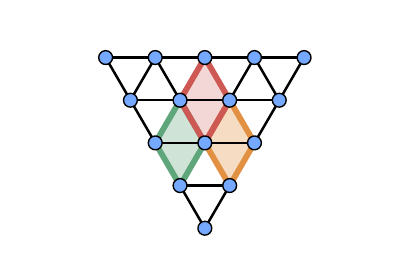
\begin{tikzpicture}[line cap=round,line join=round]
  \useasboundingbox (-2.25,-1.35) rectangle (2.25,1.35);

  \begin{scope}[scale=0.63, shift={(-2.0,-1.9)}]
    \foreach \i in {0,...,4} {
      \foreach \j in {0,...,\i} {
        \coordinate (h\i\j) at ({\j+0.5*(4-\i)},{0.86*\i});
      }
    }
    \fill[softorange!32] (h11) -- (h21) -- (h32) -- (h22) -- cycle;
    \fill[softgreen!30] (h10) -- (h20) -- (h31) -- (h21) -- cycle;
    \fill[softred!24] (h21) -- (h31) -- (h42) -- (h32) -- cycle;
    \foreach \i in {0,...,3} {
      \pgfmathtruncatemacro{\next}{\i+1}
      \foreach \j in {0,...,\i} {
        \draw[edge] (h\i\j) -- (h\next\j);
        \draw[edge] (h\i\j) -- (h\next\the\numexpr\j+1\relax);
      }
    }
    \foreach \i in {1,...,4} {
      \pgfmathtruncatemacro{\last}{\i-1}
      \foreach \j in {0,...,\last} {
        \draw[edge] (h\i\j) -- (h\i\the\numexpr\j+1\relax);
      }
    }
    \draw[softorange, line width=2.1pt] (h11) -- (h21) -- (h32) -- (h22)
      -- cycle;
    \draw[softgreen, line width=2.1pt] (h10) -- (h20) -- (h31) -- (h21)
      -- cycle;
    \draw[softred, line width=2.1pt] (h21) -- (h31) -- (h42) -- (h32)
      -- cycle;
    \foreach \i in {0,...,4} {
      \foreach \j in {0,...,\i} {
        \node[blue dot] at (h\i\j) {};
      }
    }
  \end{scope}
\end{tikzpicture}

\end{document}
